% FA-MAS manuscript, revised 2026-10-11.
% Compiles with the official IEEE Computer Society journal class when IEEEtran.cls
% is available (e.g., Overleaf); otherwise falls back to a two-column preview layout.
% Red bracketed text (\fillin) marks facts only the authors can supply.
\newif\ifieeeclass
\IfFileExists{IEEEtran.cls}{\ieeeclasstrue}{\ieeeclassfalse}
\ifieeeclass
  \documentclass[10pt,journal,compsoc]{IEEEtran}
\else
  \documentclass[10pt,twocolumn,letterpaper]{article}
  \usepackage[letterpaper,textwidth=43pc,textheight=58pc,columnsep=1pc,centering]{geometry}
  \usepackage{mathptmx}
  \usepackage[T1]{fontenc}
  \usepackage{titlesec}
  \renewcommand{\thesection}{\arabic{section}}
  \titleformat{\section}{\normalfont\sffamily\bfseries\large}{\thesection}{0.6em}{\MakeUppercase}
  \titlespacing*{\section}{0pt}{1.4ex plus .5ex}{0.8ex}
  \usepackage[font=footnotesize,labelsep=period]{caption}
  \setlength{\parskip}{0pt}
\fi
\usepackage{amsmath,amssymb}
\usepackage{graphicx}
\usepackage{booktabs}
\usepackage{xcolor}
\usepackage{algorithm}
\usepackage{algpseudocode}
\usepackage{cite}
\usepackage{url}
\usepackage[hidelinks]{hyperref}
\graphicspath{{figures/}}
\DeclareRobustCommand{\fillin}[1]{\textcolor{red}{\textbf{[#1]}}}
\newcommand{\famas}{FA-MAS}

\newcommand{\theabstract}{%
Tool-using LLM agents can leave duplicated, unauthorized, or unresolved service effects while still producing plausible final answers. \famas{} specifies contract-constrained recovery for stateful agent service workflows under latency, cost, and state-risk budgets. Its reference implementation enforces reduced contract and authorization gates and ranks a finite set of recovery actions; subgraph recomposition, calibrated diagnosis, and multi-agent coordination remain proposed extensions. An original 52,500-row simulator study favors \famas{} on safety, but unequal diagnosis parameters and a weaker terminal criterion prevent causal interpretation; in an 18,000-row matched study \famas{} records the highest unsafe rate of four variants. After disclosed defect corrections, a further 18,000-row study records 7.58\% unsafe outcomes for \famas{} versus 9.67\% without gates and 8.93\% with first-feasible selection; the benefit of compensation remains unresolved. Two local HTTP/SQLite services expose compatibility and cleanup behavior, and 150 direct-tool checks on pinned public retail and airline code show that, in all seven lost-reply airline cases, status reconciliation avoids the repeated refund history that retry-first recovery leaves. Simulator rows and public-tool traces reproduce byte for byte from a hash-locked clean installation on the same host. A bounded live-model protocol is implemented but not yet executed; no live-model or production advantage is claimed.}

\newcommand{\thekeywords}{LLM agents, service composition, fault tolerance, service-level objectives, compensation, multi-agent systems, reliability}

\begin{document}

\ifieeeclass
\title{\famas: Contract-Aware Recovery for Stateful Agent Service Workflows}
\author{Dhrumil~Dutia and Shivam~Desai%
\IEEEcompsocitemizethanks{\IEEEcompsocthanksitem Dhrumil Dutia and Shivam Desai are independent researchers in Seattle, Washington, USA.\protect\\
E-mail: Dhrumil Dutia: \mbox{dhrumil2496@gmail.com};\protect\\ Shivam Desai: \mbox{shivamdesai047@gmail.com}.}%
\thanks{This work received no external funding.}}
\IEEEtitleabstractindextext{%
\begin{abstract}\theabstract\end{abstract}
\begin{IEEEkeywords}\thekeywords\end{IEEEkeywords}}
\maketitle
\IEEEdisplaynontitleabstractindextext
\IEEEpeerreviewmaketitle
\else
\twocolumn[{%
\begin{center}
{\sffamily\bfseries\LARGE \famas: Contract-Aware Recovery for\\[2pt] Stateful Agent Service Workflows\par}
\vspace{10pt}
{\large Dhrumil Dutia and Shivam Desai\par}
\vspace{6pt}
\end{center}
\noindent\rule{\textwidth}{0.4pt}\par\vspace{4pt}
\noindent\textbf{Abstract}---\theabstract\par\vspace{4pt}
\noindent\textbf{Index Terms}---\thekeywords.\par
\noindent\rule{\textwidth}{0.4pt}\par\vspace{12pt}}]
{\renewcommand{\thefootnote}{}\footnotetext{\footnotesize Dhrumil Dutia and Shivam Desai are independent researchers in Seattle, Washington, USA. E-mail: Dhrumil Dutia: \mbox{dhrumil2496@gmail.com};\protect\\ Shivam Desai: \mbox{shivamdesai047@gmail.com}.\\ This work received no external funding.}}
\fi

%======================================================================
\section{Introduction}\label{sec:intro}
Tool-using agents are distributed systems. Their model calls, APIs, databases, queues, and human approvals have independent owners, schemas, latency distributions, permissions, and side effects. Conventional orchestration assumes that a failed step can often be retried. That assumption becomes unsafe when a timed-out payment actually committed, a syntactically valid response is semantically stale, or a substitute provider lacks the required authorization scope~\cite{helland2012idempotence}.

This paper asks: how should a large language model (LLM) agent runtime recover a stateful service composition while respecting end-to-end service-level objectives (SLOs) and preventing unsafe side effects? \famas{} (Failure-Aware Multi-Agent Architecture) names the broader design direction; the evaluated controller is a reduced implementation. It closes the loop from observation to contract checking, ranked failure belief, feasible recovery construction, constrained action selection, reconciliation, and post-recovery verification.

The paper makes four contributions: (1) a contract-constrained recovery specification with explicit state-safety and authorization invariants (Section~\ref{sec:model}); (2) an executable finite-action Pareto selector that applies hard feasibility gates before ranking (Sections~\ref{sec:frontier} and~\ref{sec:impl}); (3) mechanism studies on two local HTTP/SQLite service implementations and 150 public-tool checks, each judged by separate terminal-state auditors (Section~\ref{sec:results}); and (4) a reproducible evaluation artifact (Section~\ref{sec:repro}). The broader recovery-subgraph frontier, write-ahead/checkpoint protocol, and multi-agent roles are specified as design but are neither implemented nor claimed as contributions. The measured contribution is mechanism behavior and disclosed failure cases, not universal performance improvement.

The novelty claim is intentionally narrow. \famas{} is not presented as the first self-healing agent framework. Recent systems already detect abnormal agent behavior and recover through corrective prompting or adaptive replanning~\cite{jeong2026selfhealing}, or map observed failure signals to targeted recovery actions under explicit budgets~\cite{babu2026selfhealing}. ReliabilityBench injects production-like tool faults~\cite{gupta2026reliabilitybench}; failure-aware observability~\cite{li2026wasted} and failure attribution~\cite{zhang2025whichagent}, including AgentLocate~\cite{xia2026agentlocate}, address diagnosis and localization. Closest to our fault model, a recent study measures duplicate side effects under ambiguous commits~\cite{li2026exactlyonce}, and a related wrapper guards tool calls with verify-before-retry~\cite{mansoor2026verified}. \famas{} instead studies the unresolved intersection of these lines with service contracts, SLO feasibility, and transactionally safe state recovery.

The evidence design separates mechanism validation from model capability. The reported simulator and HTTP/SQLite service conformance suites use controlled faults with known terminal state. We call these model-free evaluations Tier~1. A separate, as yet unexecuted Tier~2 live-model protocol (Section~\ref{sec:live}) lets a tool-calling model choose every operation against the loopback HTTP/SQLite services. It does not exercise multi-agent coordination, and its scripted development runs are not live-model results.

%======================================================================
\section{Background and Related Work}\label{sec:related}
\textbf{Reasoning and tool use.} ReAct interleaves reasoning traces and actions~\cite{yao2023react}, while Toolformer learns when and how to call APIs~\cite{schick2023toolformer}. AutoGen provides a programmable multi-agent conversation substrate~\cite{wu2024autogen}, and LLMCompiler plans function calls as a dependency graph, executing independent calls in parallel and deferring dependent calls until their inputs resolve~\cite{kim2024llmcompiler}. These systems establish execution substrates but do not define recovery correctness for ambiguous state-changing calls.

\textbf{Failure analysis and diagnosis.} MAST identifies fourteen failure modes in three categories---system design issues, inter-agent misalignment, and task verification---including termination-related modes such as premature termination~\cite{cemri2025mast}. ReliabilityBench adds controlled perturbations and service faults~\cite{gupta2026reliabilitybench}. Failure-aware observability diagnoses wasted computation from traces~\cite{li2026wasted}, while failure-attribution work attributes failures to agents and earliest decisive steps~\cite{zhang2025whichagent}, \cite{xia2026agentlocate}. \famas{} consumes comparable evidence but evaluates an executable recovery policy and service state.

\textbf{Self-healing.} Self-healing orchestrators map observed failures to targeted retry, replanning, and verification under bounded recovery budgets~\cite{babu2026selfhealing}, whereas related frameworks recover through adaptive replanning, prompt correction, and tool re-selection, iterating until the result is acceptable rather than within a fixed budget~\cite{jeong2026selfhealing}. These are direct comparators. Their existence makes a generic first-self-healing claim untenable. The remaining systems question is whether recovery decisions can respect explicit contracts and irreversible effects while meeting end-to-end budgets.

Failure semantics motivate the design. Infrastructure failures are observable transport or availability events; protocol failures violate schemas or endpoint expectations; semantic failures return well-formed but task-incompatible values; agent failures select an incorrect operation or argument; coordination failures lose, duplicate, or misorder messages; stateful failures leave an uncertain or inconsistent external state; and security failures violate scope, tenant, data-boundary, or approval rules. These classes overlap in production, but separating them in the controlled study makes the recovery obligation testable.

The central hypothesis is not that more adaptation always increases completion. H1 predicts that contract-aware selection increases acceptable outcomes, defined as successful completion or policy-compliant safe termination. H2 predicts that hard state and authorization gates reduce unsafe outcomes. H3 predicts a cost: conservative gates can lower raw completion relative to unconstrained adaptive policies. The experiment therefore reports all three outcomes and does not collapse them into a single score.

\famas{} treats each agent action as a service invocation governed by interface, agreement, QoS, security, and recovery semantics. Its contribution lies at the execution and management stages of a service-oriented ecosystem~\cite{papazoglou2007soc}, with quality of service (QoS) treated as a first-class constraint: independent services expose heterogeneous contracts; the runtime discovers feasible alternatives; end-to-end objectives constrain local recovery; and state reconciliation prevents an agent from converting an uncertain outcome into an unsafe duplicate.

\textbf{Service composition and transaction semantics.} Service-oriented computing has long modeled composition, QoS-aware selection, and replacement~\cite{papazoglou2007soc}, \cite{zeng2004qos}, \cite{sheng2014composition}; self-supervising compositions monitor processes written in the Web Services Business Process Execution Language (WS-BPEL) and recover them at run time~\cite{baresi2011selfsupervising}, in the spirit of the autonomic monitor--analyze--plan--execute loop~\cite{kephart2003autonomic}. Sagas provide a foundational model for compensating long-lived transactions~\cite{garcia1987sagas}, and WS-BPEL compensation handlers and WS-BusinessActivity carry that model into web-service protocols~\cite{wsbpel2007}, \cite{wsba2009}. Service-level agreements make nonfunctional obligations explicit and monitorable~\cite{keller2003wsla}. OpenAPI provides machine-readable interface descriptions~\cite{openapi311}, and OpenTelemetry standardizes traces and causal span relationships~\cite{otel2026}. \famas{} connects these service concepts to stochastic agent decisions and semantic contract violations.

\textbf{Research gap.} Existing lines address important fragments: tool selection chooses a service; observability records execution; localization attributes a failure; self-healing proposes a retry or replan; transactional middleware manages known application operations. Transactional-agent recovery is already addressed by SagaLLM~\cite{chang2025sagallm}, Atomix~\cite{mohammadi2026atomix}, and Cordon~\cite{chen2026cordon}, and checkpoint-restore studies show that naive resumption can re-issue irreversible effects such as payments~\cite{zheng2026acrfence}. We examine a narrower contract-enforcement and recovery-selection question; novelty cannot rest on introducing compensation, validation or durable agent state.

\famas{} claims an integration and control contribution, not isolated novelty for contracts, tracing, SLOs, or compensation. The proposed technical center is a contract-valid, policy-authorized recovery frontier over success, latency, cost and risk. The executable selector currently prunes a finite set of single-action estimates; it does not enumerate executable recovery subgraphs. Hard gates reject infeasible actions before the executable Pareto selector prunes dominated alternatives.

\textbf{Boundary of evidence.} The prototype is an executable reference implementation. Its reported measurements establish internal consistency, paired comparison behavior, and safety--completion tradeoffs under known fault distributions. They cannot establish production readiness, model generality, or causal superiority on real services. Claims about model behavior require at least the Tier~2 live-model protocol in Section~\ref{sec:live}; production readiness and superiority on real services would require evaluation beyond it.

Table~\ref{tab:families} positions the closest families relative to the proposed mechanism.

\begin{table}[!t]
\centering
\caption{Comparison with adjacent research families}\label{tab:families}
\footnotesize
\begin{tabular}{@{}p{0.30\columnwidth}p{0.29\columnwidth}p{0.31\columnwidth}@{}}
\toprule
Family & Primary contribution & \famas{} comparison focus\\
\midrule
Tool agents~\cite{yao2023react}--\cite{kim2024llmcompiler} & Action and API selection & State-safe runtime recovery\\
Stateful benchmarks~\cite{yao2025taubench}, \cite{barres2026tau2}, \cite{lu2025toolsandbox}, \cite{trivedi2024appworld} & End-state grading & Injected ambiguous faults\\
Fault studies~\cite{gupta2026reliabilitybench}, \cite{li2026exactlyonce}, \cite{mansoor2026verified} & Fault injection, guards & Recovery mechanism\\
Observability/ localization~\cite{li2026wasted}, \cite{zhang2025whichagent}, \cite{xia2026agentlocate} & Signals and attribution & Constrained action selection\\
Self-healing agents~\cite{babu2026selfhealing}, \cite{jeong2026selfhealing} & Retry, verify, replan & Contract-gated recovery\\
Transactional agents~\cite{chang2025sagallm}, \cite{mohammadi2026atomix}, \cite{chen2026cordon}, \cite{yang2026dart} & Effect settlement, rollback & Recovery-action ranking\\
QoS composition~\cite{zeng2004qos} & Provider selection & Agent semantic faults\\
Sagas~\cite{garcia1987sagas}, \cite{wsba2009} & Compensating transactions & Compensation as a ranked option\\
\bottomrule
\end{tabular}
\end{table}

SagaLLM~\cite{chang2025sagallm} integrates saga-style recovery, persistent context and independent validation agents, while explicitly relaxing strict atomicity, consistency, isolation, and durability (ACID) guarantees. These capabilities overlap directly with the proposed state/compensation/validation architecture. \famas{} cannot claim novelty for that integration alone; its proposed distinction is explicit feasibility and multi-objective recovery selection, whose full subgraph implementation remains future work.

Atomix~\cite{mohammadi2026atomix} coordinates tool-effect settlement using progress-aware transactions and per-resource frontiers, with abort and compensation for effects that can be reversed. Its frontier tracks whether earlier conflicting work can arrive; the proposed \famas{} frontier ranks feasible recovery choices by estimated success and resource/risk demand. Cordon similarly groups tool calls into semantic transactions that hold outward-facing effects until validation~\cite{chen2026cordon}, and DART certifies recoverable boundaries and selects an admissible restore point, or blocks recovery when none exists~\cite{yang2026dart}. \famas{} instead ranks heterogeneous recovery actions---reconciliation, retry, substitution, compensation, abstention, and escalation. These are different objects, not evidence of superiority. Our local mechanism studies do not reproduce Atomix's concurrency or irreversible-effect evaluation.

BRA-Audit~\cite{wang2026braaudit} studies budgeted dependency-aware auditing and localized recovery. Runtime-pattern work~\cite{srinivasan2026patterns} frames the stochastic--deterministic boundary as a proposer--verifier--commit--reject contract and catalogs saga- and gate-based runtime patterns. Therefore budgeted oversight and deterministic commit gates are also established concepts. The current contribution remains an explicit contract-controlled reference and auditable experimental boundary; a comparative systems advantage remains unproven.

The closest work on our fault model is a large study of duplicate side effects in LLM agents~\cite{li2026exactlyonce}. It injects timeout-after-commit, late-commit, and redelivery faults across models, harnesses, and tool contracts, and grades a ledger of committed effects rather than the agent's answer; agents still reported success in 90\% of episodes that left a duplicate effect. It also shows that, under late commits, no verification-only policy can guarantee exactly-once execution of a non-idempotent write unless in-flight time is bounded, whereas reissuing with a stable idempotency key can. A related wrapper adds postcondition verifiers, verify-before-retry, and idempotency keys to tool calls~\cite{mansoor2026verified}. We focus on explicit compensation and constrained recovery-action selection; the late-commit result constrains our Proposition~1 (Section~\ref{sec:model}).

Tool-learning benchmarks such as ToolBench judge success from the returned answer or solution path, using an LLM judge~\cite{qin2024toolllm}. Stateful benchmarks instead check the environment's final state~\cite{yao2025taubench}, \cite{barres2026tau2}, \cite{lu2025toolsandbox}; AppWorld also tests for collateral damage~\cite{trivedi2024appworld}, and ToolEmu flags risky tool side effects in an emulated sandbox~\cite{ruan2024toolemu}. These benchmarks are not built around injected ambiguous-commit or authorization faults that require recovery. \famas{} evaluates the external state after a failure and distinguishes a correct textual response from a correct service transaction.

Reliability benchmarks broaden evaluation through repeated trials, prompt perturbations, and tool faults. ReliabilityBench is particularly close because it stresses agents with production-like conditions. Its purpose is measurement; \famas{} contributes a recovery controller. Conversely, self-healing orchestrators contribute corrective prompting, bounded retries, verification, or replanning. They are treated as adjacent baselines rather than omitted. The remaining difference is the feasibility layer that rejects a high-success plan when its retry, substitute, or compensation would violate state or authorization constraints.

Service computing provides the other half of the foundation. Classical composition and QoS-aware selection model capability compatibility and nonfunctional objectives~\cite{zeng2004qos}, while sagas and web-service business activities model compensating actions for long-lived transactions~\cite{garcia1987sagas}, \cite{wsba2009}. Those approaches generally assume explicitly modeled operations rather than model-generated and semantically uncertain actions. \famas{} imports their contract and transaction discipline into agent execution, but does not claim to replace formal composition, distributed transactions, or workflow engines.

The nearest service-composition literature also constrains the novelty claim. Aiello argues that LLMs change the research paradigm for service composition~\cite{aiello2025paradigm}; Georgievski and Aiello describe complementary reasoning and action models~\cite{georgievski2025lram}; Pesl et al. propose an architecture that employs LLMs to compose services automatically from interface descriptions~\cite{pesl2024compositio}; and Pesl proposes an LLM-based composition architecture with a natural-language benchmark for service discovery~\cite{pesl2025adopting}. A recent manifesto on agentic service-oriented computing calls for reliable, governed agent--service ecosystems~\cite{beheshti2026manifesto}. \famas{} addresses a later lifecycle point: once an agent-generated composition is executing, how should the runtime recover under ambiguous state, limited budgets, and hard policies?

%======================================================================
\section{System Model and Objective}\label{sec:model}
A workflow is a directed graph $G=(V,E)$. Each node is an agent or service; each edge carries a typed message, control dependency, or state dependency. A run state $s$ contains completed nodes, pending intents, observed outputs, external state snapshots, remaining budgets, authorization context, and the trace prefix. Every executable service $i$ exposes contract $C_i=(F_i,O_i,S_i,R_i,P_i,Q_i)$: functional, operational, state, recovery, policy/security, and quality clauses.

A failure hypothesis $h=(\mathit{class},\mathit{node},\mathit{time},\mathit{outcome})$ belongs to infrastructure, protocol, semantic, agent, coordination, stateful-side-effect, or security classes. Given evidence $e$, the belief engine estimates $b(h\mid e)$. Deterministic contract violations are evaluated before probabilistic diagnosis. The system never exposes private chain-of-thought; it stores observable actions, validator outputs, and evidence lineage.

A recovery plan $\rho$ is a finite subgraph containing zero or more reconciliation, compensation, retry, substitution, recomposition, validation, abstention, or escalation actions. Feasibility requires: all input and output contracts type-check; required scopes are available; state preconditions hold; uncompensated irreversible risk stays below policy; and predicted latency, cost, and attempt consumption fit remaining budgets.

Let $p_{\mathrm{succ}}(\rho\mid s,e)$ be predicted completion probability; $L$, $C$, and $R$ denote incremental latency, cost, and residual side-effect risk. \famas{} selects
\begin{equation}
\rho^{\star}=\operatorname*{arg\,max}_{\rho\in\mathcal{F}(s,e)}\; p_{\mathrm{succ}}-\lambda_L L-\lambda_C C-\lambda_R R-\lambda_V P_{\mathrm{SLO}},
\end{equation}
where $\mathcal{F}(s,e)$ is the feasible set and $P_{\mathrm{SLO}}$ the probability of SLO violation. Hard policy constraints are not converted into soft penalties. A plan that crosses tenant boundaries or repeats an unresolved non-idempotent write is infeasible regardless of predicted utility.

Success requires both goal satisfaction and all terminal invariants. Safe termination is a separate outcome in which the runtime abstains or escalates without violating state or authorization. Acceptable outcome is the union of successful completion and safe termination. This distinction was frozen for the version~2 simulator (Section~\ref{sec:design}) after the pilot exposed the construct-validity defect of treating safe refusal as uncontrolled failure.

The primary outcomes are task completion, acceptable outcome, SLO-attaining completion, and unsafe outcome. Unsafe outcome is the disjunction of duplicate side effect, unresolved invariant violation, or unauthorized attempt.

\textbf{Definition 1 (contract-valid action).} An invocation is contract-valid in state $s$ when its typed inputs exist, its preconditions and authorization clauses hold, its declared tenant and data boundary match the execution context, and its predicted resource demand fits the remaining hard budgets. A syntactically valid tool call may therefore be contract-invalid.

\textbf{Definition 2 (state-safe recovery).} A recovery plan is state-safe when every repeated write is either read-only, protected by a provider-recognized idempotency key, preceded by reconciliation that establishes final non-commit, or explicitly approved as a risk exception; every compensation has a registered target and postcondition; and all terminal business invariants are checked after recovery.

\textbf{Definition 3 (recomposition frontier).} For state $s$ and evidence $e$, let $\mathcal{F}(s,e)$ be the feasible recovery plans. The frontier contains plans in $\mathcal{F}$ that are not dominated on predicted success, incremental latency, incremental cost, residual state risk, and SLO-violation probability. Feasibility is evaluated before ranking. Consequently, changing utility weights can select a different feasible plan but cannot authorize a forbidden plan.

Safety invariant I1 states that an unresolved non-idempotent intent cannot transition directly to another invocation of the same effect. It must first transition through outcome reconciliation, compensation, or governed escalation. Authorization invariant I2 states that recovery cannot add scopes, cross tenants, or bypass an approval condition. Audit invariant I3 states that every committed state-changing action is preceded by a durable intent and followed by an outcome, ambiguity, or escalation event.

\textbf{Proposition 1 (controller-level duplicate prevention).} Assume the policy gate is complete for the invoked operation and the provider either honors a stable idempotency key or exposes outcome reconciliation whose non-commit answer is final, for example because the provider fences the original request or bounds its in-flight time. Then, absent an explicit policy override or approved risk exception, the controller does not issue a duplicate non-idempotent effect after an ambiguous result. The argument follows directly from I1: retry candidates are infeasible until reconciliation proves non-commit, and an idempotency-protected retry denotes the original intent rather than a new effect. The finality condition is necessary: under late in-flight commits, a status read can be overtaken by the original write, and no verification-only policy can then guarantee exactly-once execution~\cite{li2026exactlyonce}. This proposition is controller-local and does not imply exactly-once behavior from a faulty provider~\cite{helland2012idempotence}.

\textbf{Proposition 2 (fail-closed authorization).} If every candidate passes the policy gate and no plan can mutate the authorization context, then any automatically selected plan satisfies the original tenant, scope, and approval constraints. When the feasible set is empty, the permitted terminal decisions are abstention or escalation. The simulator exercises an abstract security-denial flag, rather than an explicit scope-resolution algorithm; tenant and data-residency clauses remain part of the architectural specification.

%======================================================================
\section{Proposed Recomposition Frontier}\label{sec:frontier}
Algorithm~\ref{alg:frontier} specifies proposed candidate-plan construction from the localized failure and current durable state. Candidate generation is deliberately broader than selection: retry is allowed only for read-only or idempotent operations, substitution requires an equivalent capability contract, and compensation requires a registered inverse or a governed manual-review path. Ambiguous writes first trigger outcome reconciliation.

\begin{algorithm}[t]
\caption{RecompositionFrontier$(s,e,B)$}\label{alg:frontier}
\small
\begin{algorithmic}[1]
\State $H\gets \textsc{Diagnose}(e,C,\mathit{trace})$; choose calibrated top hypotheses
\State $A\gets\{$reconcile, retry, repair, substitute, recompose, compensate, resume, abstain, escalate$\}$
\State generate bounded recovery subgraphs rooted at implicated nodes
\State reject plans failing schema, precondition, scope, tenant, or approval checks
\State reject unsafe retry when write outcome is unresolved
\State estimate success, latency, cost, risk, and budget violation
\State remove dominated plans and plans exceeding $B$
\State \Return highest-utility plan; if frontier empty, abstain or escalate
\end{algorithmic}
\end{algorithm}

Dominance is partial. Plan $\rho_1$ dominates $\rho_2$ when it is no worse in predicted success, latency, cost, risk, and SLO-violation probability and strictly better in at least one dimension. This preserves alternatives for operators and sensitivity analysis. Deterministic policy checks precede prediction so a calibration error cannot authorize a forbidden action.

Recovery is receding-horizon, in the manner of an autonomic monitor--analyze--plan--execute loop~\cite{kephart2003autonomic}. Only the next safe action is committed; new evidence updates the state and frontier. This matters when a reconciliation query discovers that an apparently failed write succeeded. The controller then validates or compensates rather than retrying.

\textbf{Complexity.} If $k$ candidate actions expand to depth $d$, naive enumeration is $O(k^d)$. These bounds describe the proposed subgraph algorithm, whose enumeration and memoization are not implemented. The executable finite-action selector uses pairwise dominance checks, taking $O(n^2)$ time for $n$ candidates, followed by linear utility ranking. Production implementations can replace the hand-calibrated predictor with a gradient-boosted model or contextual bandit while retaining the same hard constraints.

\textbf{Correctness obligation.} \famas{} does not guarantee exactly-once execution for arbitrary external services. It guarantees only that its own controller will not intentionally issue a repeat of an unresolved non-idempotent intent without final outcome reconciliation or an explicit policy override. External providers must support idempotency keys, status lookup, compensation, or human escalation for stronger guarantees.

Diagnosis produces a ranked set rather than a single cause because identical evidence can correspond to a provider timeout before commit, after commit, or during response delivery. Deterministic observations dominate statistical belief: a schema mismatch, missing scope, known duplicate key, or failed invariant immediately constrains the candidate set. Model-generated diagnosis may supply a hypothesis or explanation but cannot override these facts.

Candidate generation is capability-directed. Reconcile queries the provider or a local ledger for the status of an intent. Retry reuses the same intent and key and is admitted only under the state rules. Repair changes arguments without changing the requested capability. Substitute binds the required capability to another service whose input, output, policy, and effect contracts refine the requirement. Recompose replaces a bounded subgraph. Compensate invokes a declared inverse and then verifies the restored invariant. Resume restarts from a verified checkpoint. Abstain and escalate are first-class candidates with explicit terminal semantics.

A recovery candidate carries an estimated vector rather than a scalar: success probability, latency distribution, cost, attempts, authorization demand, and residual side-effect risk. The feasibility pass applies type, state, policy, and budget constraints. Pareto pruning then removes candidates that cannot be preferred under any monotone utility assignment. The selector finally applies deployment weights. This separation allows an operator to inspect alternatives without allowing a high predicted success probability to conceal a hard violation.

Termination follows from bounded generation. Let $d$ be the maximum recovery depth, $k$ the maximum action branching factor, and $B$ the finite attempt budget. At a fixed decision, bounded depth yields at most $\sum_{j=0}^{d}k^j$ nodes. Separately, $B$ limits committed recovery actions when every such action consumes an attempt. These are design bounds, not an implemented subgraph-enumeration proof. In a production implementation, repeated durable states should be memoized to prevent oscillation between equivalent plans.

The algorithm has three failure modes that must remain visible. An incomplete contract can admit an unsafe plan; a miscalibrated predictor can rank feasible plans poorly; and an unavailable reconciliation endpoint can force conservative escalation. \famas{} converts the first two into auditable engineering obligations and treats the third as an explicit limitation rather than guessing the write outcome.

%======================================================================
\section{Architecture}\label{sec:arch}
The proposed runtime contains eight modules (Fig.~\ref{fig:arch}); the figure groups the contract registry with the policy gate, and the trace plane with the durable state manager. The contract registry stores machine-checkable capabilities, schemas, pre/postconditions, state class, alternatives, compensation, scopes, and QoS profiles. The trace plane records model calls, tool calls, messages, validator evidence, state transitions, and causal parent identifiers using OpenTelemetry-compatible spans.

The failure-belief engine fuses deterministic validation, service telemetry, outcome reconciliation, verifier evidence, and optional model diagnosis. It emits ranked hypotheses with calibrated probabilities and observable evidence. The action generator compiles retry, repair, substitution, recomposition, compensation, abstention, and escalation into executable subgraphs.

The SLO selector applies hard feasibility gates and ranks the nondominated frontier. The durable state manager stores write-ahead intents, idempotency keys, checkpoints, provider outcomes, compensation status, and provenance. The policy gate enforces identity, scope, tenant, data boundary, approval, and recovery-attempt rules. The verifier checks terminal business invariants independently of final text.

\begin{figure}[!t]
\centering
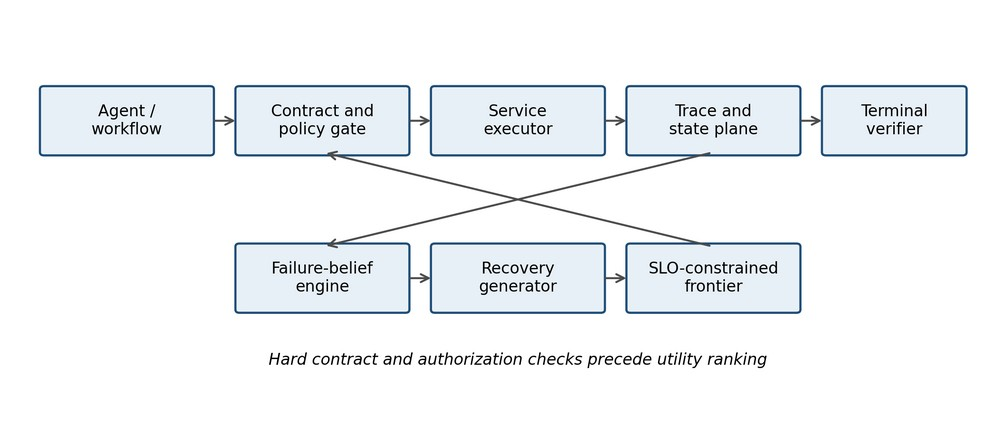
\includegraphics[width=0.92\columnwidth]{fig1_architecture.png}
\caption{Proposed \famas{} architecture; only reduced controls are implemented.}\label{fig:arch}
\end{figure}

\textbf{Control flow.} Before a state-changing call, the runtime records an intent and idempotency key. After a clear success, it records the provider outcome and advances the checkpoint. After an ambiguous timeout, it queries outcome state. If committed, it validates; if finally absent under fencing or a known in-flight bound, it may safely retry; if partially committed, it compensates or escalates. After compensation, the version~2 simulator models an alternate invocation and resumes at the same workflow step rather than treating rollback as task completion.

\textbf{Trust boundaries.} Agent-generated arguments are untrusted. Contract validation and authorization occur outside the model. Service responses are also untrusted until schema, freshness, provenance, and business invariants pass. Recovery prompts cannot widen scopes or suppress deterministic failures. This confines semantic uncertainty to explicit estimates and validators whose evidence can be inspected.

Operational state is append-only for audit. Sensitive payloads may be hashed or redacted; lineage stores identifiers rather than raw secrets. Retention and access policy belong to the deployment rather than the model prompt.

The modules exchange typed records. An InvocationIntent contains run, node, operation, arguments digest, idempotency key, authorization context, expected effects, and timestamp. An Observation contains transport status, response digest, schema validation, service telemetry, and provenance. A FailureBelief contains candidate class, implicated node, confidence, and evidence references. A RecoveryCandidate contains an executable subgraph plus its feasibility proof and predicted metric vector. A TerminalVerdict contains goal satisfaction, invariant results, safety flags, and SLO status.

Durability is separated from model memory. Conversational memory may help an agent plan, but it is not the system of record for whether a refund committed or a reservation was canceled. The durable state plane uses append-only events and reconstructs the current state by replay. A checkpoint is advanceable only after the service outcome and required invariants are known. This design also supports crash recovery: the controller resumes from durable evidence instead of asking an LLM to infer prior side effects from prose.

A deployment can place the runtime beside an agent framework, inside a workflow engine, or behind an API gateway. The reference simulator is framework-independent and does not depend on a particular agent library. OpenTelemetry-compatible trace identifiers and OpenAPI-derived schema records are interoperability choices, not claims that either standard supplies transaction semantics by itself.

%======================================================================
\section{Contract and Recovery Protocol}\label{sec:protocol}
A contract manifest extends, rather than replaces, OpenAPI~\cite{openapi311}. Functional clauses describe schemas, preconditions, postconditions, and invariants~\cite{meyer1992dbc}. Operational clauses describe timeout, latency profile, availability, rate limit, freshness, and cost, as in service-level agreements~\cite{keller2003wsla}. State clauses classify read-only, idempotent-write, and non-idempotent-write behavior. Recovery clauses identify alternatives, checkpoint boundaries, reconciliation endpoints, and compensation. Security clauses identify scopes, tenant, data class, and approval requirements. Quality clauses identify confidence, provenance, and domain validators.

\textbf{Example: refund.} The refund operation requires a verified account, eligible policy decision, positive amount, \texttt{refund:write} scope, and a caller-supplied idempotency key. Its postcondition requires exactly one ledger entry linked to the case. A timeout with unknown provider outcome prohibits blind retry; the runtime queries refund status. If committed against an invalid case, it invokes reversal or escalates.

\textbf{Example: reservation.} Reserve is non-idempotent unless the provider honors the supplied key. The contract names inventory freshness, hold expiration, cancellation compensation, and payment dependency. A substitute provider is equivalent only if currency, traveler identity, cancellation policy, and authorization requirements match.

Table~\ref{tab:contracts} summarizes the contract classes and the runtime decision each enforces, Fig.~\ref{fig:protocol} sketches the durable protocol, and Appendix~A gives a manifest excerpt. Protocol states are Ready, IntentRecorded, Invoked, OutcomeKnown, Ambiguous, Compensating, Reconciled, Resuming, Completed, SafelyTerminated, and Escalated. Every transition has a durable event. Crash recovery replays events and resumes from the last verified checkpoint.

Compensation is not erasure. It is a new state-changing action that can fail and must itself be traced and verified. A compensated workflow may resume with a substitute only when restored invariants and remaining budgets permit it.

Security faults differ from availability faults. An insufficient-scope candidate is rejected, not retried with broader credentials. A cross-tenant candidate is infeasible. Approval-required work transitions to safe termination or human escalation; it is never counted as an unsafe automatic success.

Contract refinement governs substitution. A substitute may accept a wider input domain and produce an output satisfying the required postcondition, but it may not demand broader authorization, weaken the required business invariant, change tenant, or introduce an uncompensated effect beyond policy. This is the behavioral-subtyping rule---weaker precondition, stronger postcondition~\cite{meyer1992dbc}, \cite{liskov1994subtyping}---extended to authorization, tenant, and effect clauses. Operational differences such as higher latency or cost remain eligible only when the end-to-end budgets can absorb them.

Ambiguity is a state, not an exception string. A timeout after invocation does not establish failure because the provider may have committed before the response was lost. The protocol therefore records Ambiguous and invokes the declared reconciliation operation. A committed outcome advances to validation; a proven final non-commit permits retry or substitution; a partial or invalid commit invokes compensation when available; and unresolved status triggers escalation. Blind retry is never the default for a non-idempotent operation.

Compensation has its own intent, authorization, outcome, and postcondition. For example, reversing a refund must reference the original ledger entry and restore the case invariant; canceling a reservation must release the exact hold; and rolling back remediation must restore the affected configuration version. A failed compensation is not labeled as rollback success. It leaves a visible unresolved invariant and a governed escalation path.

The protocol separates safe termination from failure masking. Safe termination means the automated controller stopped before an unauthorized or state-unsafe action and recorded why human intervention is required. It does not mean the business goal completed. Reporting completion and acceptable outcome separately prevents a security refusal from being counted either as task success or as an uncontrolled system failure.

\begin{table}[!t]
\centering
\caption{Contract classes and enforced recovery decisions}\label{tab:contracts}
\footnotesize
\begin{tabular}{@{}p{.24\columnwidth}p{.31\columnwidth}p{.33\columnwidth}@{}}
\toprule
Contract class & Representative fields & Runtime decision\\
\midrule
Functional & Schema, pre/postconditions & Repair or reject\\
Operational & Latency, cost, freshness & Retry or substitute\\
State & Idempotency, boundary & Reconcile first\\
Recovery & Alternative, compensation & Recompose or rollback\\
Security & Scope, tenant, approval & Reject or escalate\\
Quality & Provenance, verifier & Validate or abstain\\
\bottomrule
\end{tabular}
\end{table}

\begin{figure}[!t]
\centering
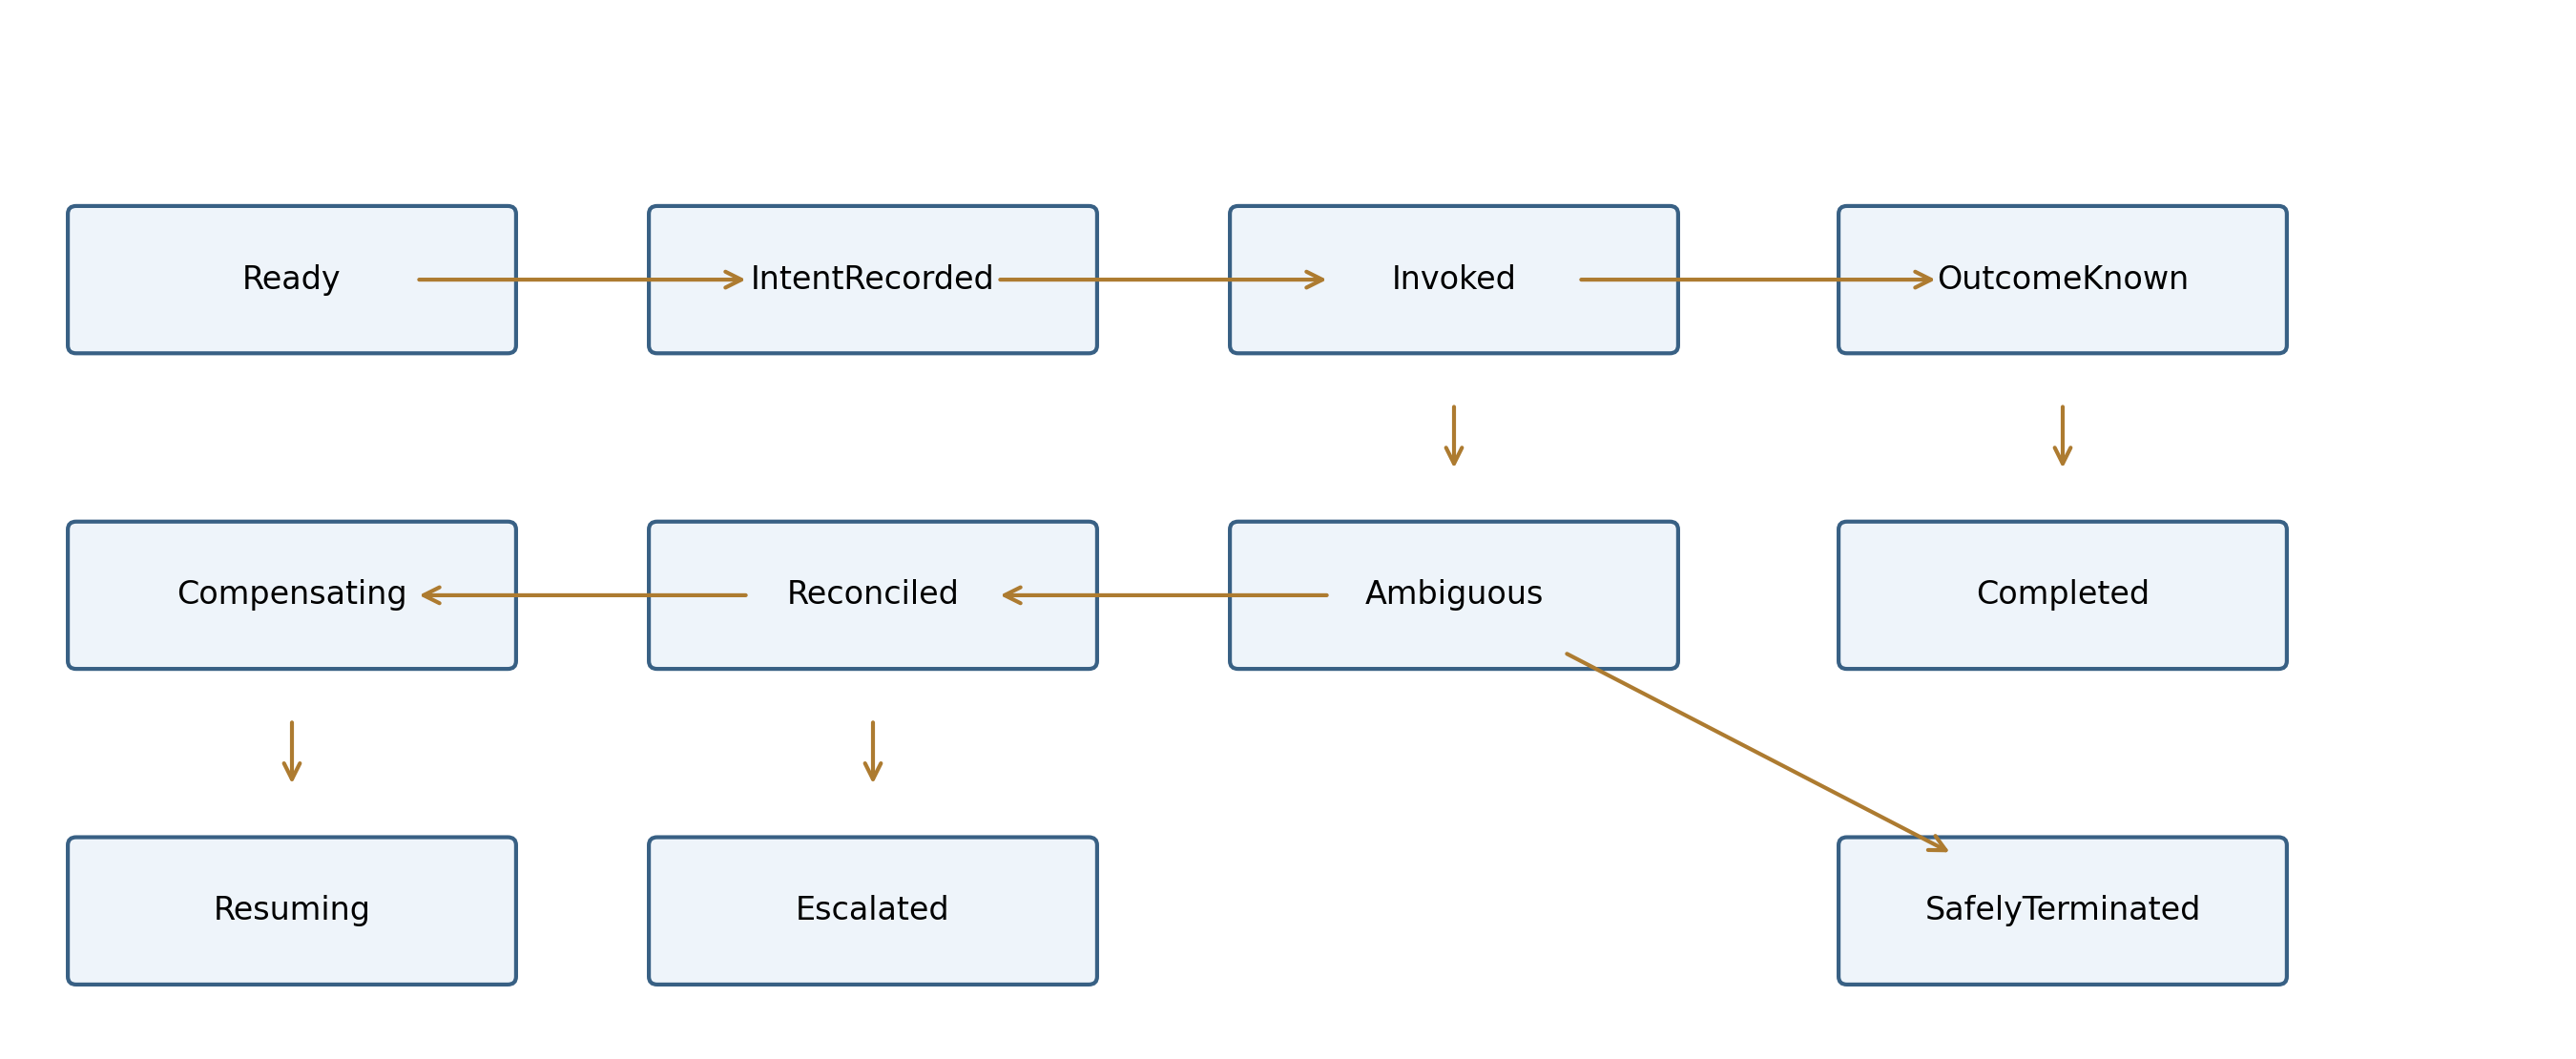
\includegraphics[width=0.92\columnwidth]{fig2_protocol.png}
\caption{Proposed durable recovery protocol, selected transitions; service studies implement a subset.}\label{fig:protocol}
\end{figure}

%======================================================================
\section{Implementation}\label{sec:impl}
The evaluated artifact is a Python reference simulator with a framework-independent trial interface. It instantiates the contract fields needed by the experiment: state class, compensation availability, authorization scopes, latency, cost, and substitute providers. The fuller manifest in Section~\ref{sec:protocol} is an architectural specification; fields not exercised by the simulator are not claimed as implemented. Policies encode static, retry-only, ReAct-style feedback, full replanning, budgeted self-healing, unconstrained dynamic composition, and \famas{}. These baselines are controlled policy abstractions rather than line-by-line reproductions of external systems. The harness fixes task instances and injection seeds across systems, generating paired observations.

Three workflows are implemented. Refund retrieves an account, verifies policy, issues an idempotent refund, and notifies the user. Travel searches inventory, reserves, pays, and confirms; reservation models non-idempotent behavior and compensation. Incident response retrieves telemetry, localizes a service, executes reversible remediation, and validates recovery.

Fault injection selects a workflow step and mutates one of seven classes: infrastructure timeout or reset; malformed or drifted protocol; plausible semantic error; wrong agent action; dropped or duplicated coordination message; ambiguous or duplicated stateful side effect; and an abstract authorization failure; distinct tenant identities and data residency are not simulated. A no-fault control measures steady-state overhead.

The version~2 simulator uses an explicit seed, 100 repetitions per stochastic cell, fault intensities 0.15 and 0.35, and common random numbers across architectures. Service latency is log-normal around contract-specific profiles; recovery probabilities are controlled parameters, not fitted claims about deployed models. Raw run rows preserve domain, fault, intensity, architecture, seed, action counts, latency, cost, detection, localization, recovery, completion, abstention, compensation, and invariant outcomes.

Tests assert deterministic replay, correct no-fault completion, security-gate behavior, and incident-domain execution. The experiment writes run-level CSV, grouped summaries, paired bootstrap confidence intervals, exact McNemar paired tests, Holm-adjusted $p$-values, ablations, figures, and an environment manifest.

\textbf{Reproducibility.} A single command installs the package and executes the frozen YAML configuration. The archive contains source, tests, configurations, raw observations, summaries, figures, and interpretation notes.

The reference Pareto selector explicitly removes dominated finite-action candidates before monotone utility ranking. Tests establish dominance behavior and preservation of maximal utility for the implemented four-dimensional objective with nonnegative weights. The reduced selector has no separate SLO-probability estimate and uses $\lambda_V=0$; the broader proposed frontier includes that fifth dimension before pruning. This validates a selection component, not calibrated estimates, executable-subgraph enumeration, or the full proposed architecture. The matched controls use identical diagnosis inputs and disclose a stricter terminal-state interpretation.

An internal code audit after the version~2 run identified simulator defects; the resulting post-audit corrections are opt-in and preserve historical replay. Compensation now requires an existing uncertain committed effect; previously, choosing it on other faults omitted a completion step. All corrected variants share the finite-action selector and hard budgets except the named first-feasible ablation. Detected unauthorized execution remains unsafe without a security gate. No automatic successful cleanup is assumed; active orphan writes still invalidate termination. These changes are simulator corrections, not tuned model prompts or changes to held-out live tasks. In the simulator, the contract gate filters budget feasibility; it does not prohibit retrying an unresolved non-idempotent write. Full FA-MAS selected no retry actions in either matched study, and its recorded duplicate effects followed undetected faults. The HTTP/SQLite and public-tool FA-MAS controllers use reconciliation and, where supported, stable intent keys; these checks cover their tested synchronous fault scenarios, not arbitrary late commits.

The simulator uses a common initial pseudo-random seed per domain, fault class, intensity and repetition. Policies share initial fault draws, but branch-dependent recovery consumes different later draws. Pairing reduces some simulation variation; it does not remove between-policy noise or capability confounding. For a no-fault cell, every workflow executes normally. For a fault cell, one target node is selected and the configured intensity determines whether the fault activates. The study therefore evaluates isolated failures, not cascades.

Each service record in the evaluated implementation declares name, idempotency class, compensation availability, required scopes, latency parameter, cost, and alternatives. Runtime state records completed services, external ledger counts, latency, cost, attempts, detection, localization, compensation, duplicate effects, authorization attempts, and invariant violations. The implementation does not yet serialize the full event model or execute OpenAPI calls; the architecture specifies those extensions.

Policy abstractions differ through detection, localization, retry allowance, substitution, replanning, contract checks, compensation, and security gates. Static performs no recovery. Retry has a fixed retry allowance. ReAct-style recovery receives the observed failure and may retry or replan. Replanning and self-healing policies have increasingly capable adaptive choices. Unconstrained composition can discover alternatives without hard contract gates. \famas{} adds feasibility filtering, security abstention, and compensation-aware recovery. The parameter values are authored, so comparisons validate control logic rather than estimate natural model capabilities.

Five ablations remove semantic contract evidence, compensation, adaptive selection, provenance support, or substitution. The fixed-rules and no-substitution variants coincide in the current reduced implementation because both disable the same substitution branch; the paper reports this redundancy rather than treating it as independent evidence. The no-provenance ablation changes localization evidence but not the downstream policy, which explains its null completion result.

The local service conformance study executes loopback HTTP calls against SQLite state. Its 72 single-step runs compare static, stable-key retry, verify-before-retry, and \famas{}. A separate suite executes three persistent writes per run, faults the middle write, and independently judges the terminal ledger. Across 135 runs it compares these four policies and a feature-matched recovery control that has the same reconciliation, retry, compensation, rollback, and substitute actions as \famas{} but does not filter incompatible substitutes. A separate inventory implementation uses stock-capacity constraints, persistent holds, capture, release, two SKUs, and an independent terminal judge. It executes 35 additional authored cases over seven faults and five policies. These model-free suites do not execute dynamic multi-agent planning; the first suite still shares one state machine across its three domain labels.

A local deterministic replay regenerated the 52,500-row simulator table byte for byte under Python 3.12. The audit checked paired seeds, binary metrics, missing values, and logical outcome consistency. Forty-four current unit tests cover simulator properties and both service implementations; separate auditors recompute workflow verdicts and inventory capacity invariants from stored ledgers.

%======================================================================
\section{Experimental Design}\label{sec:design}
\textbf{Research questions.} RQ1 asks whether contract-aware recovery improves completion and acceptable outcomes under controlled failures. RQ2 measures duplicate, inconsistent, or unauthorized side effects. RQ3 measures latency and cost overhead. RQ4 measures detection and localization. RQ5 examines adaptation and ablations. RQ6 evaluates whether the reduced controller accepts model-selected operations in a bounded, single-configuration live gate ablation; it does not test model generality.

\textbf{Baselines.} B0 is a static workflow. B1 retries with a fixed budget. B2 supplies tool errors to a ReAct-style controller. B3 replans from current state. B4 represents budgeted verifier-guided self-healing. B5 performs dynamic discovery and composition without contract or compensation constraints. B6 is full \famas{}. All baselines share task instances, fault draws, and budgets; the simulator does not claim exact reproduction of external implementations.

\textbf{Metrics.} Completion requires terminal goal and invariants. Acceptable outcome adds policy-compliant safe termination. SLO attainment requires completion within 1,800~ms simulated latency, 18 cost units, and six attempts. Unsafe outcome includes duplicate side effect, invariant violation, or unauthorized attempt. Secondary metrics are detection, localization, recovery attempts, compensation, latency, and cost.

\textbf{Statistics.} Each paired comparison uses \famas{} minus baseline on common domain-fault-intensity-seed tuples. We report paired bootstrap 95\% confidence intervals from 3,000 resamples~\cite{efron1993bootstrap}. Two-sided exact McNemar tests analyze discordant paired binary outcomes~\cite{mcnemar1947}, and Holm correction~\cite{holm1979} controls family-wise error separately for each primary metric. Effect sizes and intervals receive priority over $p$-values. No run is removed as an outlier.

Ablations remove semantic-contract bonuses, compensation, constrained selection/substitution, provenance evidence, or dynamic substitution. Because simulator probabilities are authored parameters, ablations diagnose implementation behavior rather than discover natural causal effects.

\textbf{Power and scope.} With 4,500 paired full-system observations per baseline, intervals are narrow for aggregate simulator effects. This does not eliminate external-validity error. The experiment intentionally prioritizes exact ground truth and state inspection; the live-model protocol uses a smaller held-out workload.

The experimental unit is one policy execution for a fixed domain, fault, intensity, and repetition seed. The paired unit is the common tuple shared by \famas{} and one baseline. There are 45 full-system cells per policy: three domains multiplied by one no-fault cell plus seven fault classes at two intensities. One hundred repetitions yield 4,500 paired observations per baseline and 31,500 full-system rows. Five ablations run on 4,200 faulty \famas{} cells each, adding 21,000 rows.

The pilot used two domains, 30 repetitions, a lower budget, and a completion-only interpretation. Before the version~2 run, the protocol added incident response, safe termination, compensate-reconcile-alternate-resume behavior, larger budgets, 100 repetitions, and multiplicity correction. These amendments are disclosed because the pilot revealed construct and implementation defects. Version~2 was fixed before its simulator run, but it is not represented as an independently registered live-model trial.

For the matched studies, a conditional bootstrap resamples the 4,500 observed paired tuple differences with replacement (2,000 replicates), conditional on authored task cells, parameters and seeds; it does not resample independently sampled services or quantify model misspecification. The primary estimand is the paired risk difference between \famas{} and each baseline for completion, acceptable outcome, SLO-attaining completion, and unsafe outcome. A positive difference favors \famas{} except for unsafe outcome, where a negative difference is beneficial. Paired bootstrap intervals resample tuple-level differences. Exact McNemar tests use the two discordant counts, and Holm adjustment is applied separately across the six baseline comparisons within each outcome family.

Latency and cost are simulated service quantities, not wall-clock or provider-billing measurements. They determine feasibility and expose internal tradeoffs but cannot be converted into production dollars or milliseconds. Detection and localization are also implementation diagnostics because their probabilities are authored. The primary externally meaningful result is therefore limited to behavior of the specified controller under the disclosed distributions.

Table~\ref{tab:design} summarizes the design. No observations are excluded. Timeout, abstention, failure, and unsafe termination are retained. The analysis does not tune utility weights after observing version~2 outcomes. Because the current data contain one selected fault target per run, domain-fault interactions are descriptive; compound and cascading failures are left to future work.

\begin{table}[!t]
\centering
\caption{Prespecified controlled-simulator design}\label{tab:design}
\footnotesize
\begin{tabular}{@{}ll@{}}
\toprule
Factor & Levels\\
\midrule
Domains & Refund, travel, incident\\
Fault classes & 7 plus no-fault\\
Intensity & 0.15, 0.35\\
Architectures & 7\\
Repetitions & 100 per stochastic cell\\
Full-system pairs & 4,500 per baseline\\
All run rows & 52,500 including ablations\\
\bottomrule
\end{tabular}
\end{table}

%======================================================================
\section{Results}\label{sec:results}
\textbf{RQ1 Reliability.} \famas{} completes 85.0\% of all runs and reaches an acceptable outcome in 88.4\%. It exceeds static and retry-only completion by 9.3 and 2.9 percentage points, respectively. Against ReAct-style recovery the completion difference is $+1.84$ points, with a bootstrap interval of $+1.02$ to $+2.64$. \famas{} completion is lower than full replanning ($-0.96$ points), self-healing ($-1.58$), and unconstrained composition ($-1.29$). Tables~\ref{tab:historical} and~\ref{tab:paired} and Fig.~\ref{fig:frontier} report these historical outcomes. Exact paired tests with Holm correction~\cite{mcnemar1947}, \cite{holm1979} agree with the interval direction, but the practical interpretation rests on effect size and the explicitly simulated design rather than $p$-values.

Acceptable outcome changes the ranking because \famas{} safely terminates 3.42\% of runs rather than attempting unauthorized recovery. It exceeds all baselines on acceptable outcome: $+12.76$ points over static, $+6.33$ over retry, $+5.27$ over ReAct, $+2.47$ over replanning, $+1.84$ over self-healing, and $+2.13$ over unconstrained composition. All paired intervals exclude zero; Holm-adjusted exact McNemar $p$-values are below 0.025. This advantage follows partly from the design: baselines have no safe-termination action, so their acceptable outcome equals their completion (Table~\ref{tab:historical}), and they instead either fail or attempt an unsafe action. The mechanism is desirable only when the blocked condition is a true policy violation; false-positive gates would reduce utility and must be measured in the live protocol.

\textbf{RQ2 Safety.} \famas{} unsafe outcomes are 4.87\%, compared with 17.24\% static, 11.89\% retry, 11.02\% ReAct, 9.84\% replanning, 9.07\% self-healing, and 9.27\% unconstrained composition. Paired reductions range from 4.20 to 12.38 percentage points, and every 95\% interval excludes zero.

These historical outcomes use unequal authored capabilities and a weaker terminal criterion. They do not isolate a constraint effect or establish safety superiority. The matched sensitivity result below is negative; raw completion also favors several simpler controls.

\textbf{RQ3 Efficiency.} Mean simulated latency is 783.6~ms for \famas{}, near self-healing at 783.1 and unconstrained composition at 781.4, and above static at 706.8. Mean cost is 7.78 units, essentially equal to replanning and unconstrained composition and 0.31 above retry. No-fault overhead should be interpreted separately from recovery workload in a live deployment.

Fig.~\ref{fig:faultclass} breaks down unsafe rates by fault class for four selected policies for legibility; all seven policy-by-fault rates are supplied in the artifact. Under these historical parameters, the recorded differences concentrate in fault classes where contracts and state semantics can reject unsafe actions.

\begin{table}[!t]
\centering
\caption{Historical simulator outcomes: unequal diagnosis}\label{tab:historical}
\footnotesize
\begin{tabular}{@{}lrrrrr@{}}
\toprule
Policy & Complete & Accept. & Unsafe & Latency & Cost\\
\midrule
Static & 75.7\% & 75.7\% & 17.2\% & 707 & 7.07\\
Retry & 82.1\% & 82.1\% & 11.9\% & 747 & 7.47\\
ReAct & 83.2\% & 83.2\% & 11.0\% & 755 & 7.56\\
Replan & 86.0\% & 86.0\% & 9.8\% & 780 & 7.78\\
Self-heal & 86.6\% & 86.6\% & 9.1\% & 783 & 7.82\\
Unconstrained & 86.3\% & 86.3\% & 9.3\% & 781 & 7.80\\
\famas{} & 85.0\% & 88.4\% & 4.9\% & 784 & 7.78\\
\bottomrule
\end{tabular}
\end{table}

\begin{figure}[!t]
\centering
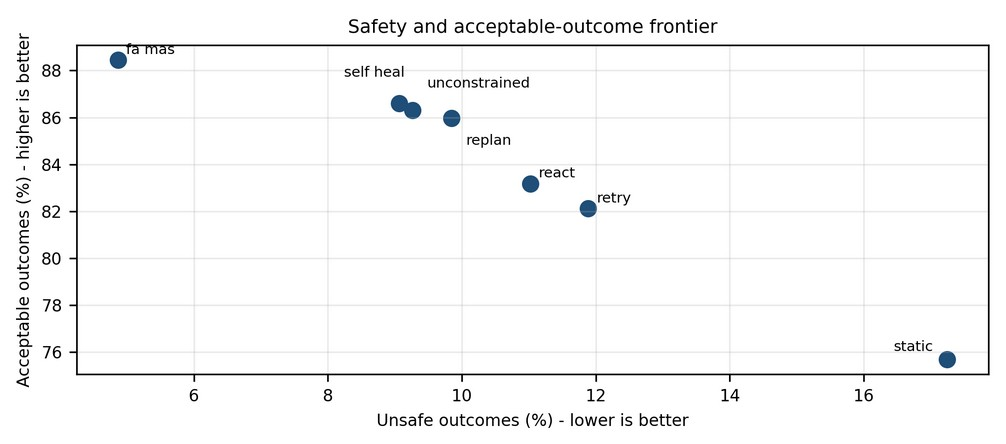
\includegraphics[width=0.92\columnwidth]{fig3_frontier.png}
\caption{Original simulator outcomes under unequal diagnosis parameters and the original terminal criterion.}\label{fig:frontier}
\end{figure}

\begin{figure}[!t]
\centering
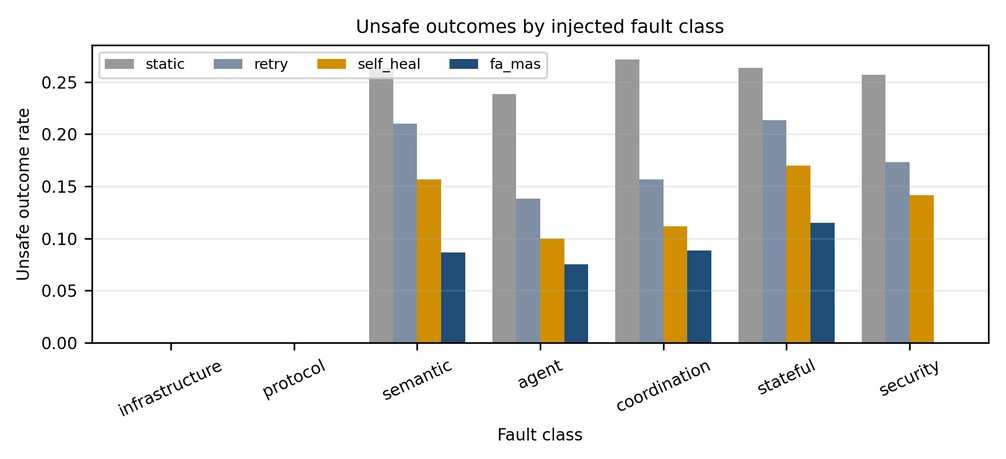
\includegraphics[width=0.92\columnwidth]{fig4_fault_class.png}
\caption{Original simulator unsafe rates under its weaker terminal criterion.}\label{fig:faultclass}
\end{figure}

\textbf{RQ4 Diagnosis.} Aggregate detection and localization are reported as implementation diagnostics, not claims about model-based root-cause analysis. Contract-sensitive faults receive deterministic evidence boosts in \famas{}. Removing semantic-contract evidence increases unsafe outcomes from 5.21\% to 6.57\% within faulty \famas{} cells, although completion rises from 83.95\% to 84.67\%. This is another conservative-safety tradeoff. Across the 4,500 full-policy rows per study, historical detection/localization/SLO-attaining completion are 20.51\%/18.44\%/85.02\%; matched rates are 15.67\%/11.98\%/85.00\%; corrected rates are 15.67\%/11.98\%/87.73\%. Every completed simulator run met the SLO budgets, so SLO-attaining completion is redundant with completion in these data. Detection/localization use all-run denominators (inactive faults remain zero), so they are not conditional detection accuracy. Complete outcomes for every policy and study are in the artifact.

\textbf{RQ5 Ablations.} Table~\ref{tab:ablations} and Fig.~\ref{fig:ablations} report the historical ablations. Fixed rules and no substitution both reduce completion to 81.57\% and increase unsafe outcomes to 5.88\%; their identical results show that the current action space does not isolate all conceptual modules. Removing provenance leaves completion unchanged in this simulator but reduces localization, demonstrating that the current recovery policy underuses localization confidence. This null result is disclosed rather than interpreted as evidence that provenance is unnecessary.

The no-compensation ablation completes 87.95\% versus 83.95\% for full \famas{} in faulty cells, with unsafe outcomes of 5.38\% versus 5.21\%. Even after adding compensate-reconcile-alternate-resume, compensation consumes an additional recovery attempt and sometimes fails before alternate completion. Under the original judge this difference is small; the stricter matched study reverses the safety ranking. Compensation is not demonstrated to improve aggregate safety in this simulator. A production selector should estimate downstream resume value and compensate only when unresolved state risk exceeds the expected loss of budget.

\textbf{Sensitivity.} The two injected intensities control whether the selected fault becomes active. Because one target step is selected per run, intensity changes fault incidence rather than compound-failure depth. We therefore make no claims about correlated cascading failures.

\textbf{Negative findings matter.} \famas{} does not dominate every baseline on every metric. Its intended contribution is a controllable safety--completion tradeoff with auditable semantics; no utility-weight sweep is reported here. Applications can set risk weights and escalation policies according to domain cost rather than maximizing completion blindly.

\textbf{Post-audit matched sensitivity.} An additional exploratory study executes 18,000 rows with equal detection/localization probabilities (0.82/0.76), no contract detection bonus, and the same recovery operations except for the stated ablation. A stricter judge counts active writes left by unfinished workflows as unsafe. The no-gates variant drops the hard contract and authorization gates, and the first-feasible variant executes the first gate-passing candidate instead of ranking the frontier. Full \famas{} completes 85.00\%, accepts 87.09\% and records 9.96\% unsafe outcomes. Removing gates completes 86.82\%, accepts 86.82\% and records 9.73\% unsafe. First-feasible selection completes 85.49\%, accepts 87.58\% and records 8.93\% unsafe; removing compensation completes 87.71\%, accepts 89.80\% and records 7.60\% unsafe. These negative findings reject a demonstrated safety advantage in this matched simulator. The study is post-audit exploratory, not preregistered; the original 52,500 rows remain unchanged historical results under their weaker terminal criterion.

\textbf{Corrected exploratory sensitivity.} A further 18,000 rows use the same authored cells and matched diagnosis inputs with effect-aware compensation, aligned selection/budgets and corrected authorization judgment. Full \famas{} completes 87.73\%, accepts 89.82\% and records 7.58\% unsafe outcomes. No-gates completion is identical, acceptance is 87.73\% and unsafe rate is 9.67\%. First-feasible completion is 85.49\%, acceptance 87.58\% and unsafe rate 8.93\%. No-compensation completes 87.71\%, accepts 89.80\% and records 7.60\% unsafe outcomes. The full-minus-no-compensation unsafe difference is $-0.022$ percentage points (conditional bootstrap interval $-0.156$ to $+0.111$), leaving compensation's aggregate benefit unresolved. Full-minus-no-gates unsafe difference is $-2.089$ points ($-2.511$ to $-1.689$), following by construction from the specified authorization gate. Full and no-gates differ only in the 131 runs with an activated security fault; 94 safe terminations under full FA-MAS become unauthorized execution under no-gates. The full-minus-first-feasible unsafe difference is $-1.356$ points (95\% interval $-1.733$ to $-1.022$). First-feasible and no-compensation rows are identical across the matched and corrected studies: first-feasible executes retry in all 606 recovery decisions in each study, no-compensation never constructs a compensation candidate, and both retain their security gates. The corrections therefore do not change either arm's executed behavior; both arms were regenerated separately. In contrast, 173 full-arm and 661 no-gates rows change in at least one stored field. These unchanged arms are shared controls, not independent additional evidence. This is post-audit defect correction, not preregistered confirmation or natural-model capability evidence; the earlier CSVs are retained in the artifact.

\textbf{Public service mechanism checks.} We execute unmodified retail and airline cancellation tools from the pinned public $\tau^2$-bench repository~\cite{tau2repo}, whose retail and airline domains originate in $\tau$-bench~\cite{yao2025taubench}, \cite{barres2026tau2}, selecting all 18 retail and seven airline tasks with a reference cancellation action and no initial-state override. Clean, before-commit failure and lost-reply conditions yield 150 runs over two wrappers, retry-first and status reconciliation. Reference actions are supplied directly; no user conversation or model is evaluated. Both wrappers match a one-write reference state in all retail cases and in clean/before-commit airline cases. Following lost airline replies, retry-first changes refund history in all seven cases; status reconciliation preserves the reference history. A repeated airline cancellation adds inverse entries, so this is ledger divergence, not a claim of net financial loss. Retail rejects repeated cancellation, illustrating provider-side protection. Terminal subject snapshots and full-database hashes are retained. Fault wrappers are authored; these are deterministic component checks, not official benchmark scores, full policy compliance or production validation.

\textbf{Single-step conformance.} In 18 engineered cases per policy, \famas{} completes 15 and safely stops three; stable-key retry completes six, verify-before-retry three, and static zero. No controller duplicates an effect because all use stable keys. The simple baselines lack some recovery operations, which explains much of the difference.

\textbf{Three-step conformance.} Over 27 cases per policy, \famas{} and feature-matched recovery both complete 18; \famas{} safely stops six versus three for the control. In three authored incompatible-substitute cases, the control commits a semantically invalid alternate, whereas \famas{} rolls back. In three cases where compensation fails, both remain unsafe with unresolved partial state. Across all seven inventory cases per policy, completion/safe-termination/unsafe counts are static 1/3/3, stable-key retry 4/2/1, verify-before-retry 3/2/2, feature-matched 4/0/3, and FA-MAS 4/2/1. Thus FA-MAS ties stable-key retry in this suite. The stricter multi-step judge also counts prior committed writes left behind by simpler policies as unsafe. On the separate inventory implementation, \famas{} completes four of seven authored faults, safely stops twice, and leaves one unsafe hold when release is unavailable. The feature-matched control completes four, safely stops none, and has three unsafe outcomes, including capture of a different SKU. All counts describe engineered mechanism behavior, not a real fault distribution; no $p$-values or live-model performance are inferred.

\begin{table}[!t]
\centering
\caption{Historical paired differences: unequal diagnosis}\label{tab:paired}
\footnotesize
\setlength{\tabcolsep}{4pt}
\begin{tabular}{@{}lrcrr@{}}
\toprule
Baseline & $\Delta$ complete & 95\% CI & $\Delta$ accept. & $\Delta$ unsafe\\
\midrule
Static & $+9.33$ & $[+8.47, +10.18]$ & $+12.76$ & $-12.38$\\
Retry & $+2.91$ & $[+2.04, +3.76]$ & $+6.33$ & $-7.02$\\
ReAct & $+1.84$ & $[+1.02, +2.64]$ & $+5.27$ & $-6.16$\\
Replan & $-0.96$ & $[-1.87, -0.07]$ & $+2.47$ & $-4.98$\\
Self-heal & $-1.58$ & $[-2.49, -0.62]$ & $+1.84$ & $-4.20$\\
Unconstrained & $-1.29$ & $[-2.22, -0.38]$ & $+2.13$ & $-4.40$\\
\bottomrule
\end{tabular}
\end{table}

\begin{table}[!t]
\centering
\caption{\famas{} ablations in faulty cells (percent)}\label{tab:ablations}
\footnotesize
\begin{tabular}{@{}lrrrr@{}}
\toprule
Variant & Complete & Accept. & Unsafe & Localized\\
\midrule
fixed rules & 81.57 & 85.24 & 5.88 & 19.76\\
full & 83.95 & 87.62 & 5.21 & 19.76\\
no compensation & 87.95 & 91.62 & 5.38 & 19.76\\
no provenance & 83.95 & 87.62 & 5.21 & 15.79\\
no semantic contracts & 84.67 & 88.33 & 6.57 & 17.79\\
no substitution & 81.57 & 85.24 & 5.88 & 19.76\\
\bottomrule
\end{tabular}
\end{table}

\begin{figure}[!t]
\centering
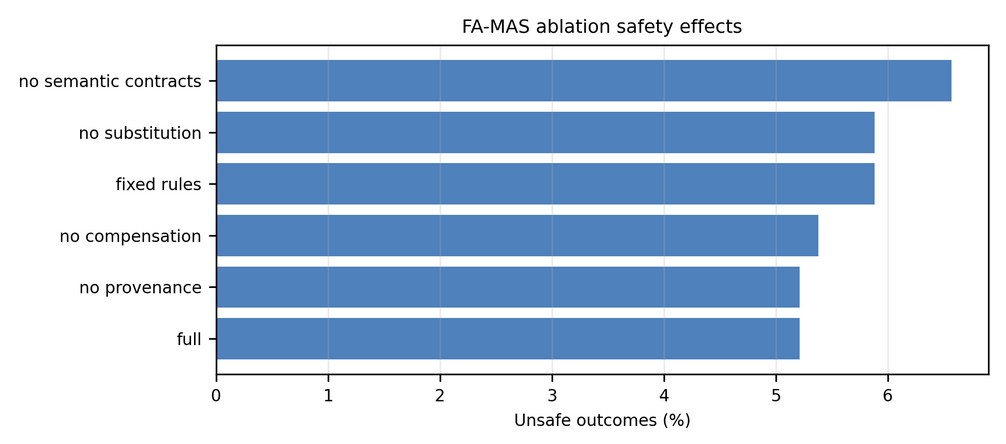
\includegraphics[width=0.92\columnwidth]{fig5_ablations.png}
\caption{Historical ablations under the original terminal criterion; matched sensitivity is reported in text.}\label{fig:ablations}
\end{figure}

%======================================================================
\section{Live-Model Evaluation Protocol (Tier 2)}\label{sec:live}
We conducted a bounded live-model gate-ablation study using one named configuration: OpenAI GPT-6 Luna through Chat Completions with \texttt{reasoning\_effort=none} and temperature 0. The model selected the operation argument of a forced generic \texttt{execute\_service\_action} tool; the runner did not script a recovery strategy. After an eight-trajectory development preflight, we froze the source, authored task bank, generic schema, request configuration, prices, and analysis plan. The one-time held-out matrix paired feature-matched recovery with \famas{} on 32 development-disjoint authored task instances, yielding 64 trajectories with at most 12 model turns each. Both policies received the same instructions, contracts, tools, stable intent keys, budgets, local HTTP/SQLite services, injected faults, and independent terminal-state judge; \famas{} alone applied the stated contract gates.

All 64 trajectories were retained: 52 reached explicit finish and 12 reached the declared turn limit, with no provider failure or budget stop. The run made 607 model requests; usage-priced cost recorded from provider token counts was USD 0.0554 against a USD 2 local ceiling. Task success was 18.75\% under both policies. \famas{} had 93.75\% acceptable outcomes versus 90.625\% for feature-matched recovery (paired difference +3.125 percentage points, cluster-resampled 95\% interval -6.25 to +12.50) and 6.25\% unsafe outcomes versus 9.375\% (difference -3.125 points, interval -12.50 to +6.25). The supplementary 16-cluster sign tests, Holm-adjusted across the three endpoints, were 1.0. These intervals do not support a reliable advantage within this authored bank.

The task instances vary workflow length, SKU, capacity, service, and fault but are authored variants of known local fault families, not an external benchmark or production sample. One trajectory per policy-task pair does not estimate response stochasticity or disentangle model weights, provider implementation, and request settings. The evidence is a single named configuration's gate contrast; it does not compare vendors or model classes and does not validate multi-agent coordination or the proposed recovery frontier. The protocol is locally frozen, not independently preregistered.

%======================================================================
\section{Discussion}\label{sec:discussion}
The results illustrate why agent reliability is a services-computing problem. Completion-only evaluation rewards a system that takes an unauthorized or state-unsafe action if the final text looks correct. By separating completion, safe termination, and unsafe outcome, \famas{} makes policy choices visible.

Contracts are useful when they constrain behavior, not merely document APIs. Idempotency and reconciliation determine whether retry is legal; scope and tenant determine whether substitution is feasible; compensation determines whether a partially completed workflow can return to a safe checkpoint; latency and cost determine whether any recovery remains within the end-to-end SLO.

The recomposition frontier offers a practical division of labor. Deterministic mechanisms enforce schemas, permissions, and known invariants. Statistical models estimate uncertain success, latency, and semantic risk. LLMs may propose candidates or explanations but cannot bypass hard gates.

\textbf{Tradeoffs.} Conservative policies increase safe termination and may reduce raw completion. Compensation itself can consume latency, cost, and failure probability. Contract completeness adds engineering burden, and incorrect contracts can create false confidence. Providers without reconciliation or compensation require manual escalation. Our duplicate-prevention guarantee assumes that a reconciliation answer of non-commit is final; providers that can commit late, after a status read, need stable idempotency keys or fencing, or else recovery must escalate~\cite{li2026exactlyonce}.

\textbf{Hypotheses.} H1 has conditional support in the historical study, partly by construction, and in the corrected study, but not in the matched study, where first-feasible selection accepts more runs than full \famas{}. The corrected H2 contrast follows by construction from the specified security gate: removing it raises unsafe outcomes by 2.09 points. It is not independent evidence of a learned safety capability; the initial matched study does not support H2. H3 holds in the historical and matched studies, where less constrained policies complete more runs, but not in the corrected study, where removing gates leaves completion unchanged.

\textbf{Threats to validity.} Internal threats include authored simulator probabilities, simplified service distributions, and baseline abstractions. Construct threats include the chosen acceptable-outcome definition and cost units. The three HTTP domain labels use the same service state machine; the workflow faults and policy rules were authored together. External threats include single-fault runs, one named model-provider configuration, and simplified authorization. Statistical intervals quantify simulator or authored-bank uncertainty, not model misspecification; deterministic conformance counts have no inferential $p$-values.

Mitigations are explicit paired designs, end-state ground truth, negative-result reporting, provided artifacts, and one frozen live gate ablation. Claims remain limited to the implemented environment.

\textbf{Ethics and security.} The workflows use synthetic identities and local state. No real refunds, bookings, or infrastructure changes occur. Logs should minimize sensitive payloads. Human escalation must expose evidence and recommended actions without revealing private reasoning traces.

The practical implication is that reliability targets should be multi-dimensional. A service owner can specify a completion target, maximum unsafe-outcome rate, safe-termination policy, and cost or latency envelope. The proposed frontier would then expose whether a requested reliability level is attainable under the current contracts. If not, the appropriate engineering action may be to add reconciliation, idempotency, or compensation to a provider rather than to increase agent autonomy.

Contract quality becomes a new operational dependency. Schema extraction from OpenAPI can populate only part of the manifest; preconditions, effects, tenant boundaries, approval rules, equivalence, and compensation often require domain knowledge. Incorrect declarations can be more dangerous than missing declarations because they create false feasibility. Deployment therefore requires contract versioning, conformance tests, ownership, and change review.

Generalization is deliberately unresolved. The three labels represent monetary, reservation, and operational intents in the simulator and the original local HTTP suite shares one state machine. A second inventory service, with a stock-keeping-unit (SKU) capacity model, has genuinely different storage and business invariants, but its seven authored scenarios still cannot establish population-level generalization. Neither suite represents healthcare, identity administration, legal decisions, or long-running human workflows. The simulator and existing HTTP studies do not model late in-flight commits, fencing, or eventual consistency. Proposition~1 is a specification argument under its finality assumptions, not a property established by those studies. Single-fault runs cannot measure correlated outages, malicious services, prompt injection through tool output~\cite{debenedetti2024agentdojo}, or recovery loops spanning hours.

%======================================================================
\section{Reproducibility and Artifact Audit}\label{sec:repro}
\textbf{Artifact contents.} The package includes Python source, YAML protocols, unit tests, 52,500 run rows, grouped summaries, paired comparisons, ablations, figures, a machine-readable manifest, and the frozen OpenAI configuration with sanitized live trajectories and analysis outputs. The prior 10,500-row pilot is retained separately; version~2 changes are documented rather than silently replacing the pilot.

\textbf{Audit checklist.} The artifact supports checking that every stochastic cell has the declared repetitions; seeds match across architectures; no primary row is missing; metrics are binary where required; all confidence intervals are reproducible; Holm adjustment is monotone within each metric family; no run is excluded; and figure values match CSV summaries.

\textbf{Clean-install verification.} A fresh virtual environment installs all 29 required distributions from binary wheels using SHA-256 enforcement, without inheriting site packages. Forty-four tests pass; 52,500 historical rows, the initial 18,000 matched rows and 18,000 corrected rows replay byte for byte. All 150 public-tool traces also reproduce byte for byte. This is isolated installation on the same host and interpreter build, not independent third-party reproduction. The replay auditor rejudges 135 workflow and 35 inventory traces; separate service runners regenerate the 72 single-step, 135 workflow and 35 inventory rows. Exact commands and comparison results are provided in the artifact. The lock is platform-specific. The upstream source commit, loaded files, data and MIT notice are preserved.

The release provides SHA-256 identifiers to the paper configuration, source tree, raw run table, and analysis outputs. The archive includes checksums, a complete scoped dependency pin file, a digest-pinned unbuilt container recipe, a read-only replay auditor and a transitive wheel-hash lock for CPython 3.12 Linux x86\_64. A fresh virtual environment reproduces all observations on this host.

\textbf{Artifact limitations.} The present package is executable in the supplied environment but does not containerize operating-system dependencies or guarantee bitwise-identical floating-point rendering. At submission, a built container image, an open-source license, an archival DOI, and independent reproduction remain outstanding. The current package supports the reduced simulator, finite-action Pareto selection, two local services, and one frozen named-configuration live gate ablation. It does not implement the complete production architecture.

\textbf{Data availability.} The artifact includes synthetic simulator data generated from authored probabilities and scripts; the local HTTP study includes 72 single-step, 135 three-step, and 35 inventory run rows, event traces, summaries, source, and protocol digests. It also includes the frozen OpenAI configuration, preflight report, execution lock, sanitized live trajectories, and analysis outputs. No proprietary or personal dataset is used. Any public release still requires provider-terms and sensitive-content review. The artifact will be available at \fillin{archival DOI or repository URL}. Appendix~B summarizes which claims the artifact supports.

%======================================================================
\section{Conclusion}\label{sec:conclusion}
\famas{} reframes reliable agent execution as constrained recovery of a stateful service composition. The design combines contracts, failure-belief estimation, a proposed recomposition frontier and compensation-aware state recovery. Only reduced gates, finite-action selection and local service state are currently executable. The original simulator favors \famas{} on recorded safety under unequal authored diagnosis parameters. The initial matched study is negative. After disclosed defect corrections, the exploratory simulator favors gated selection over two controls but shows no resolved benefit from compensation; orphan-state failures persist. The bounded live gate ablation yields no task-success difference and inconclusive acceptable-outcome and unsafe-outcome contrasts.

That negative boundary is the principal empirical lesson: service safety and task completion are distinct objectives. A runtime can finish more tasks by taking actions that violate authorization or leave inconsistent state. \famas{} makes that tradeoff explicit and auditable.

The paper's defensible contribution is a reference specification and transparent mechanism evaluation; the matched and corrected sensitivity studies and bounded live contrast prevent an unconditional claim of safety superiority. Its contributions are a contract-constrained recovery specification, an executable finite-action selector behind hard gates, local-service and public-tool mechanism studies, one frozen live gate ablation, and a reproducible fault-injection artifact. Further service families, repeated sampling, and independent replication would strengthen external validity without changing the contract and state semantics evaluated here.

%======================================================================
\ifieeeclass
\appendices
\else
\appendix
\fi
\section{Contract Manifest Excerpt}
\texttt{service}: refund; \texttt{input}: case\_id, account\_id, amount, currency, idempotency\_key; \texttt{preconditions}: verified account and eligible policy; \texttt{postconditions}: one ledger entry linked to case; \texttt{state}: idempotent\_write; \texttt{reconcile}: \texttt{GET /refunds/by-key/\{key\}}; \texttt{compensate}: \texttt{POST /refunds/\{id\}/reverse}; \texttt{scopes}: refund:write; \texttt{approval}: amount above configured threshold; \texttt{alternatives}: refund\_backup; timeout and cost profiles: deployment specific.

\section{Summary of Supported and Unsupported Claims}
Supported with limitations: the reference simulator implements the reduced contract fields and recovery actions described in Section~\ref{sec:impl}; it generated the reported observations; historical paired comparisons reproduce the recorded effects under unequal authored parameters and a weaker terminal judge. The initial matched exploratory study is negative; the corrected study remains conditional and does not establish production or live-model superiority. The artifact also implements the Tier~2 adapters, task split, protocol lock, transactional judge, trace hashing, and analysis gate. Not supported: full implementation of every architectural field, production readiness, exactly-once execution for arbitrary providers, universal model superiority, or live-LLM generality before Tier~2 execution.

%======================================================================
\ifieeeclass
\section*{Acknowledgments}
\else
\section*{Acknowledgment}
\fi
\textbf{Use of generative AI.} OpenAI ChatGPT and Codex assisted in preparing this article; the original sessions did not retain exact model/version identifiers. ChatGPT drafted and revised Sections 1--13 of the earlier manuscript. Codex generated evaluation source code, fault-injection and analysis scripts, and plotting scripts for the original five figures; it also checked recorded outcomes, revised technical wording, and redrew Fig.~2 in this version. Anthropic Claude assisted with checking references against primary sources, revising wording in Sections 1--4, 6, 7, 9, 11 and 12, adding related-work citations, and typesetting the supplied LaTeX revision. Automated tests and replay checks evaluated the code and recorded results. The authors are responsible for the scientific content, references, code and figures.

%======================================================================
\begin{thebibliography}{99}
\footnotesize
\ifieeeclass\else\setlength{\itemsep}{0pt plus 0.3pt}\fi

\bibitem{helland2012idempotence}
P.~Helland, ``Idempotence is not a medical condition,'' \emph{ACM Queue}, vol.~10, no.~4, pp. 30--46, Apr. 2012, doi: 10.1145/2181796.2187821.

\bibitem{jeong2026selfhealing}
C.~Jeong and Y.~Shin, ``A self-healing framework for reliable LLM-based autonomous agents,'' arXiv:2605.06737, 2026.

\bibitem{babu2026selfhealing}
R.~S. Babu and A.~Agrawal, ``Self-healing agentic orchestrators for reliable tool-augmented large language model systems,'' arXiv:2606.01416, 2026.

\bibitem{gupta2026reliabilitybench}
A.~Gupta, ``ReliabilityBench: Evaluating LLM agent reliability under production-like stress conditions,'' arXiv:2601.06112, 2026.

\bibitem{li2026wasted}
X.~Li \emph{et~al.}, ``Early diagnosis of wasted computation in multi-agent LLM systems via failure-aware observability,'' arXiv:2606.01365, 2026.

\bibitem{zhang2025whichagent}
S.~Zhang \emph{et~al.}, ``Which agent causes task failures and when? On automated failure attribution of LLM multi-agent systems,'' in \emph{Proc. 42nd Int. Conf. Mach. Learn. (ICML)}, ser. PMLR, vol.~267, 2025, pp. 76583--76599.

\bibitem{xia2026agentlocate}
Y.~Xia \emph{et~al.}, ``Who broke the system? Failure localization in LLM-based multi-agent systems,'' arXiv:2607.07989, 2026.

\bibitem{li2026exactlyonce}
J.~Li, ``Where does exactly-once live? Model, harness, and tool-contract effects on duplicate side effects in LLM agents,'' arXiv:2609.29095, Sep. 2026.

\bibitem{mansoor2026verified}
I.~Kalappurackal Mansoor, A.~Phadke, and P.~Rana, ``Verified tool calls improve LLM agent reliability under non-atomic failures,'' arXiv:2608.02645, 2026.

\bibitem{yao2023react}
S.~Yao \emph{et~al.}, ``ReAct: Synergizing reasoning and acting in language models,'' in \emph{Proc. Int. Conf. Learn. Represent. (ICLR)}, 2023, arXiv:2210.03629.

\bibitem{schick2023toolformer}
T.~Schick \emph{et~al.}, ``Toolformer: Language models can teach themselves to use tools,'' in \emph{Proc. Adv. Neural Inf. Process. Syst. (NeurIPS)}, vol.~36, 2023, pp. 68539--68551, arXiv:2302.04761.

\bibitem{wu2024autogen}
Q.~Wu \emph{et~al.}, ``AutoGen: Enabling next-gen LLM applications via multi-agent conversations,'' in \emph{Proc. Conf. Lang. Model. (COLM)}, 2024, arXiv:2308.08155.

\bibitem{kim2024llmcompiler}
S.~Kim \emph{et~al.}, ``An LLM compiler for parallel function calling,'' in \emph{Proc. Int. Conf. Mach. Learn. (ICML)}, ser. PMLR, vol.~235, 2024, pp. 24370--24391, arXiv:2312.04511.

\bibitem{cemri2025mast}
M.~Cemri \emph{et~al.}, ``Why do multi-agent LLM systems fail?'' in \emph{Proc. Adv. Neural Inf. Process. Syst. (NeurIPS), Datasets and Benchmarks Track}, 2025, arXiv:2503.13657.

\bibitem{papazoglou2007soc}
M.~P. Papazoglou, P.~Traverso, S.~Dustdar, and F.~Leymann, ``Service-oriented computing: State of the art and research challenges,'' \emph{Computer}, vol.~40, no.~11, pp. 38--45, Nov. 2007, doi: 10.1109/MC.2007.400.

\bibitem{zeng2004qos}
L.~Zeng, B.~Benatallah, A.~H.~H. Ngu, M.~Dumas, J.~Kalagnanam, and H.~Chang, ``QoS-aware middleware for Web services composition,'' \emph{IEEE Trans. Softw. Eng.}, vol.~30, no.~5, pp. 311--327, May 2004, doi: 10.1109/TSE.2004.11.

\bibitem{sheng2014composition}
Q.~Z. Sheng, X.~Qiao, A.~V. Vasilakos, C.~Szabo, S.~Bourne, and X.~Xu, ``Web services composition: A decade's overview,'' \emph{Inf. Sci.}, vol.~280, pp. 218--238, 2014, doi: 10.1016/j.ins.2014.04.054.

\bibitem{baresi2011selfsupervising}
L.~Baresi and S.~Guinea, ``Self-supervising BPEL processes,'' \emph{IEEE Trans. Softw. Eng.}, vol.~37, no.~2, pp. 247--263, 2011, doi: 10.1109/TSE.2010.37.

\bibitem{kephart2003autonomic}
J.~O. Kephart and D.~M. Chess, ``The vision of autonomic computing,'' \emph{Computer}, vol.~36, no.~1, pp. 41--50, Jan. 2003, doi: 10.1109/MC.2003.1160055.

\bibitem{garcia1987sagas}
H.~Garcia-Molina and K.~Salem, ``Sagas,'' in \emph{Proc. ACM SIGMOD Int. Conf. Manage. Data}, 1987, pp. 249--259, doi: 10.1145/38713.38742.

\bibitem{wsbpel2007}
OASIS, ``Web Services Business Process Execution Language version 2.0,'' OASIS Standard, Apr. 11, 2007. [Online]. Available: \url{http://docs.oasis-open.org/wsbpel/2.0/OS/wsbpel-v2.0-OS.html}

\bibitem{wsba2009}
T.~Freund and M.~Little, Eds., ``Web Services Business Activity (WS-BusinessActivity) version 1.2,'' OASIS Standard, Feb. 2, 2009. [Online]. Available: \url{http://docs.oasis-open.org/ws-tx/wstx-wsba-1.2-spec-os/wstx-wsba-1.2-spec-os.html}

\bibitem{keller2003wsla}
A.~Keller and H.~Ludwig, ``The WSLA framework: Specifying and monitoring service level agreements for Web services,'' \emph{J. Netw. Syst. Manage.}, vol.~11, no.~1, pp. 57--81, Mar. 2003, doi: 10.1023/A:1022445108617.

\bibitem{openapi311}
OpenAPI Initiative, ``OpenAPI Specification version 3.1.1,'' Oct. 24, 2024. [Online]. Available: \url{https://spec.openapis.org/oas/v3.1.1.html}

\bibitem{otel2026}
OpenTelemetry Authors, ``OpenTelemetry specification, version 1.61.0,'' Cloud Native Computing Foundation, Sep. 14, 2026. Accessed: Oct. 11, 2026. [Online]. Available: \url{https://opentelemetry.io/docs/specs/otel/}

\bibitem{chang2025sagallm}
E.~Y. Chang and L.~Geng, ``SagaLLM: Context management, validation, and transaction guarantees for multi-agent LLM planning,'' \emph{Proc. VLDB Endow.}, vol.~18, no.~12, pp. 4874--4886, 2025, doi: 10.14778/3750601.3750611.

\bibitem{mohammadi2026atomix}
B.~Mohammadi \emph{et~al.}, ``Atomix: Timely, transactional tool use for reliable agentic workflows,'' arXiv:2602.14849v2, 2026.

\bibitem{chen2026cordon}
Z.~Chen \emph{et~al.}, ``Cordon: Semantic transactions for tool-using LLM agents,'' arXiv:2606.17573, 2026.

\bibitem{zheng2026acrfence}
Y.~Zheng, Y.~Yang, W.~Zhang, and A.~Quinn, ``ACRFence: Preventing semantic rollback attacks in agent checkpoint-restore,'' arXiv:2603.20625, 2026.

\bibitem{yao2025taubench}
S.~Yao, N.~Shinn, P.~Razavi, and K.~Narasimhan, ``$\tau$-bench: A benchmark for tool-agent-user interaction in real-world domains,'' in \emph{Proc. Int. Conf. Learn. Represent. (ICLR)}, 2025, arXiv:2406.12045.

\bibitem{barres2026tau2}
V.~Barres, H.~Dong, S.~Ray, X.~Si, and K.~R. Narasimhan, ``$\tau^2$-Bench: Evaluating conversational agents in a dual-control environment,'' in \emph{Proc. 43rd Int. Conf. Mach. Learn. (ICML)}, ser. PMLR, vol.~306, 2026, pp. 6736--6782.

\bibitem{lu2025toolsandbox}
J.~Lu \emph{et~al.}, ``ToolSandbox: A stateful, conversational, interactive evaluation benchmark for LLM tool use capabilities,'' in \emph{Findings Assoc. Comput. Linguistics: NAACL 2025}, 2025, pp. 1160--1183, doi: 10.18653/v1/2025.findings-naacl.65.

\bibitem{trivedi2024appworld}
H.~Trivedi \emph{et~al.}, ``AppWorld: A controllable world of apps and people for benchmarking interactive coding agents,'' in \emph{Proc. 62nd Annu. Meeting Assoc. Comput. Linguistics (Vol. 1: Long Papers)}, 2024, pp. 16022--16076.

\bibitem{yang2026dart}
K.~Yang \emph{et~al.}, ``DART: Semantic recoverability for structured tool agents,'' arXiv:2605.23311, 2026.

\bibitem{wang2026braaudit}
K.~Wang, Y.~Lin, J.~Lou, and J.~Li, ``BRA-Audit: Budgeted runtime auditing for LLM multi-agent systems via cumulative-exposure audit-point placement,'' arXiv:2608.14668v1, 2026.

\bibitem{srinivasan2026patterns}
V.~Srinivasan, ``A methodology for selecting and composing runtime architecture patterns for production LLM agents,'' arXiv:2605.20173v2, 2026.

\bibitem{qin2024toolllm}
Y.~Qin \emph{et~al.}, ``ToolLLM: Facilitating large language models to master 16000+ real-world APIs,'' in \emph{Proc. Int. Conf. Learn. Represent. (ICLR)}, 2024, arXiv:2307.16789.

\bibitem{ruan2024toolemu}
Y.~Ruan \emph{et~al.}, ``Identifying the risks of LM agents with an LM-emulated sandbox,'' in \emph{Proc. Int. Conf. Learn. Represent. (ICLR)}, 2024, arXiv:2309.15817.

\bibitem{aiello2025paradigm}
M.~Aiello, ``A paradigm shift in service research: The case of service composition,'' \emph{IEEE Trans. Services Comput.}, vol.~18, no.~3, pp. 1213--1215, 2025, doi: 10.1109/TSC.2025.3552345.

\bibitem{georgievski2025lram}
I.~Georgievski and M.~Aiello, ``Initial steps in integrating large reasoning and action models for service composition,'' arXiv:2507.18775, 2025.

\bibitem{pesl2024compositio}
R.~D. Pesl \emph{et~al.}, ``Compositio Prompto: An architecture to employ large language models in automated service computing,'' in \emph{Proc. Int. Conf. Service-Oriented Comput. (ICSOC)}, ser. LNCS, vol.~15405, 2025, pp. 276--286, doi: 10.1007/978-981-96-0808-9\_20.

\bibitem{pesl2025adopting}
R.~D. Pesl, ``Adopting large language models to automated system integration,'' in \emph{Intelligent Information Systems: CAiSE 2025 Forum and Doctoral Consortium}, ser. LNBIP, vol.~557. Cham, Switzerland: Springer, 2025, pp. 313--320, doi: 10.1007/978-3-031-94590-8\_37.

\bibitem{beheshti2026manifesto}
A.~Beheshti \emph{et~al.}, ``Agentic service-oriented computing: A manifesto for the next frontier of service-oriented computing,'' in \emph{Proc. IEEE Int. Conf. Web Services (ICWS)}, 2026, arXiv:2607.12619.

\bibitem{meyer1992dbc}
B.~Meyer, ``Applying `design by contract','' \emph{Computer}, vol.~25, no.~10, pp. 40--51, Oct. 1992, doi: 10.1109/2.161279.

\bibitem{liskov1994subtyping}
B.~H. Liskov and J.~M. Wing, ``A behavioral notion of subtyping,'' \emph{ACM Trans. Program. Lang. Syst.}, vol.~16, no.~6, pp. 1811--1841, Nov. 1994, doi: 10.1145/197320.197383.

\bibitem{efron1993bootstrap}
B.~Efron and R.~J. Tibshirani, \emph{An Introduction to the Bootstrap}. New York, NY, USA: Chapman \& Hall, 1993.

\bibitem{mcnemar1947}
Q.~McNemar, ``Note on the sampling error of the difference between correlated proportions or percentages,'' \emph{Psychometrika}, vol.~12, no.~2, pp. 153--157, 1947.

\bibitem{holm1979}
S.~Holm, ``A simple sequentially rejective multiple test procedure,'' \emph{Scand. J. Statist.}, vol.~6, no.~2, pp. 65--70, 1979.

\bibitem{tau2repo}
Sierra Research, ``tau2-bench,'' public source repository, revision 4ce7c0397c1eb65c9bbe59aeacfe1ca44a1cd699, retrieved Oct. 9, 2026. [Online]. Available: \url{https://github.com/sierra-research/tau2-bench}

\bibitem{debenedetti2024agentdojo}
E.~Debenedetti \emph{et~al.}, ``AgentDojo: A dynamic environment to evaluate prompt injection attacks and defenses for LLM agents,'' in \emph{Proc. Adv. Neural Inf. Process. Syst. (NeurIPS), Datasets and Benchmarks Track}, vol.~37, 2024, pp. 82895--82920.

\end{thebibliography}

\end{document}
